\subsection{McCulloch-Pitts-Neuron }

\begin{frame}
\frametitle{Zusammenhang - Biologisches Neuron}

\begin{figure}
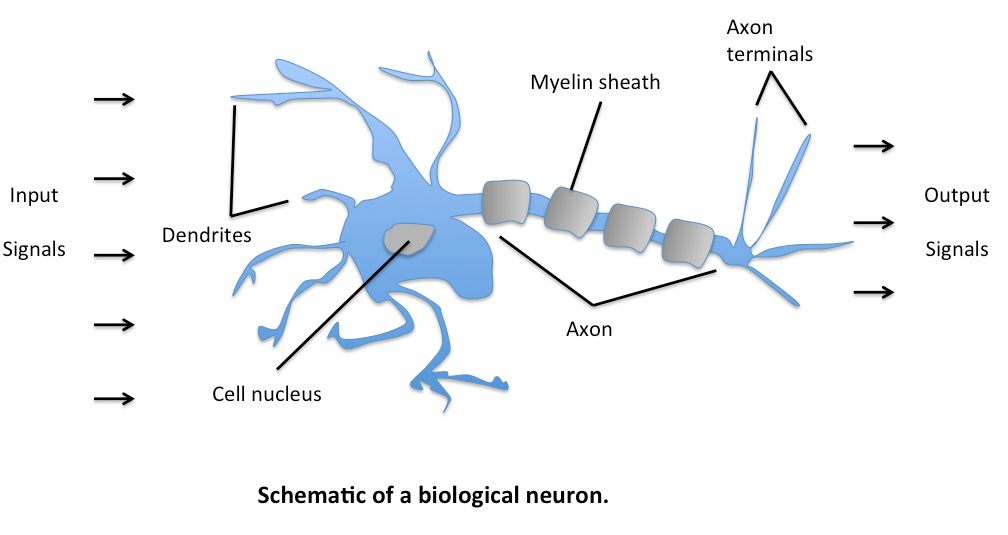
\includegraphics[width=\linewidth]{./geschichtliches/mcCullochPittsNeuron/img/bioNeuron_alpha}
\end{figure}

\end{frame}


\begin{frame}
\frametitle{MP-Neuron}

\begin{columns}

\column{0.5\textwidth}
\begin{itemize}
	\item Modell soll Funktionalität des biologischen Neurons imitieren
	\item Klassifizierungsproblem als grundlegende Problemstellung
	\item Lineare Entscheidungsfunktion zur binären Klassifizierung verwendet
\end{itemize}


\column{0.5\textwidth}
\begin{figure}
	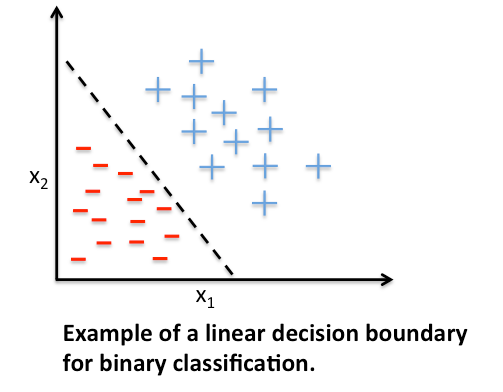
\includegraphics[width=\linewidth]{./geschichtliches/mcCullochPittsNeuron/img/bnKlassifizierung_alpha}
\end{figure}

\end{columns}

\end{frame}


\begin{frame}
\frametitle{Aufbau und Funktionsweise}
\begin{figure}
	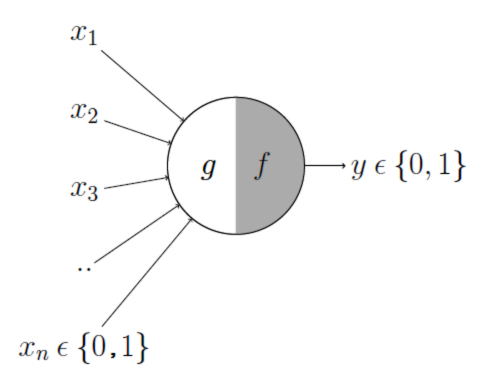
\includegraphics[width=.5\linewidth]{./geschichtliches/mcCullochPittsNeuron/img/aufbau_alpha}
\end{figure}

\hrule

\begin{columns}

\column{0.4\textwidth}
\begin{align*}
g(x_1, x_2, \dots , x_n) = g(x) = \sum_{i=1}^n x_i
\end{align*}

\column{0.4\textwidth}
\begin{align*} \label{eq:aktFkt2}
f(g(x)) =\begin{cases}
	1 & \mbox{if } g(x) \geq \theta \\
    0 & \mbox{if } g(x) < \theta
  \end{cases}
\end{align*}
\end{columns}
\end{frame}


\begin{frame}
\frametitle{Notation AND-Gatter}

\begin{figure}
	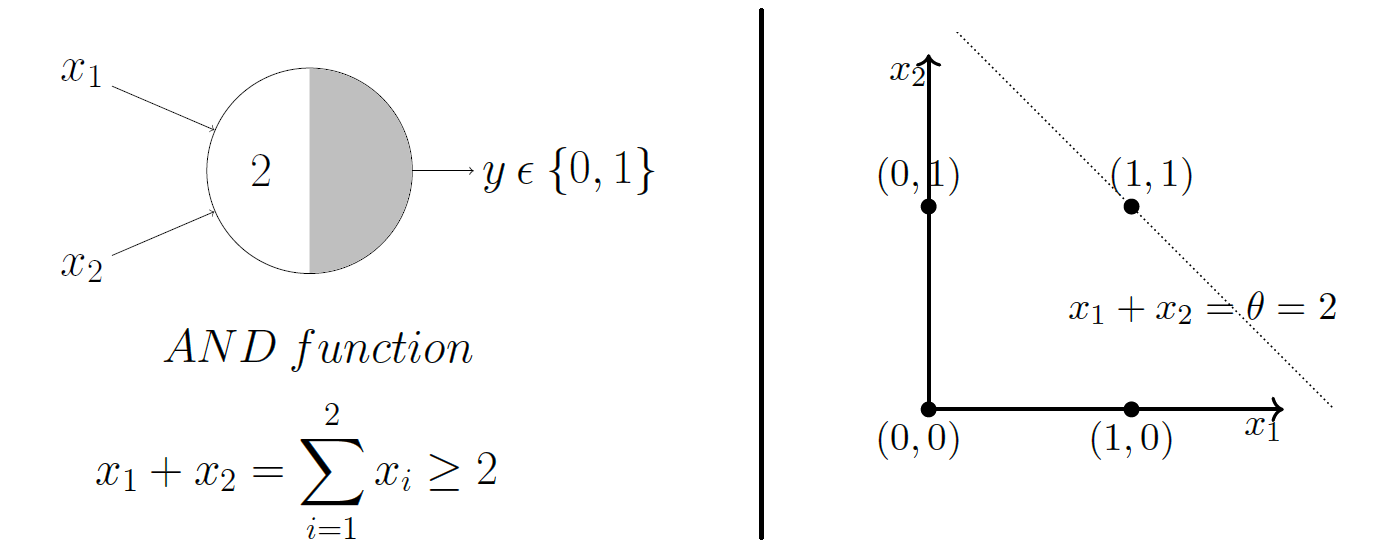
\includegraphics[width=\linewidth]{./geschichtliches/mcCullochPittsNeuron/img/mpn_and_alpha}
\end{figure}
\end{frame}


\begin{frame}
\frametitle{Notation OR-Gatter}

\begin{figure}
	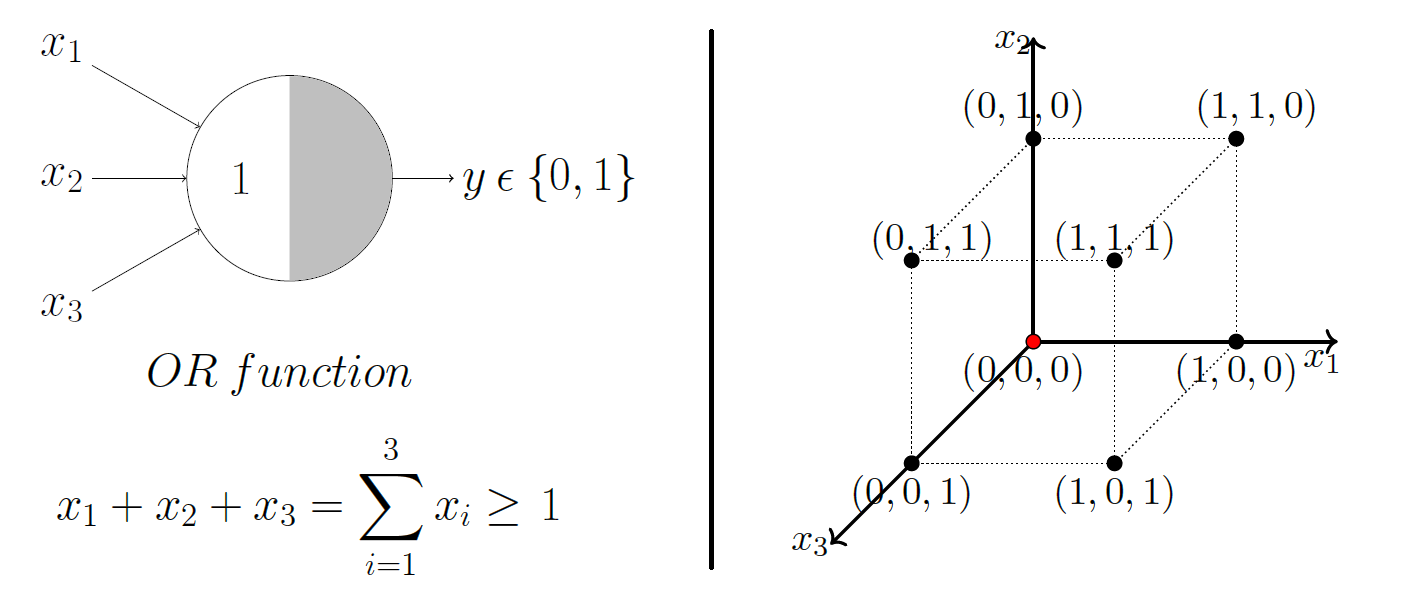
\includegraphics[width=\linewidth]{./geschichtliches/mcCullochPittsNeuron/img/mpn_or_alpha}
\end{figure}
\end{frame}


\begin{frame}
\frametitle{Nachteile}

\begin{itemize}
\item Keine kontinuierlichen Eingabewerte (nur boolesche Werte)
\item Schwelle muss manuell gesetzt werden, keine automatische Aktualisierung vorgesehen
\item Keine Priorisierungsmöglichkeit der Eingabewerte möglich
\item Funktionen müssen durch lineare Entscheidungsfunktion getrennt werden können
\end{itemize}

\end{frame}
